\chapter{Partie 1} % Depth 0

\section{Contrainte Budgétaire} % Depth 1

Modèle économique du consommateur : suppose que les individus choisissent ce qu'il y a de meilleur parmi ce qu'ils peuvent acquérir $\Rightarrow$ les consommateurs choisissent le panier qu'ils préfèrent dans leur ensemble budgétaire.
\begin{itemize}
\item[$\rightarrow$] un consommateur ne peut pas dépenser plus que sa richesse. Ce qu'il dépense = quantités qu'il achète $*$ le prix.
\item[$\rightarrow$] Il n'y a pas de place pour effectuer des prêts ou économiser de l'argent.
\end{itemize}

\textbf{La richesse du consommateur est :}
\begin{itemize}
\item soit une richesse exogène (en dehors) au modèle
\item soit la valeur de son panier initial
\end{itemize}

\subsection{Ensemble budgétaire} % Depth 2

L'ensemble budgétaire correspond à l'ensemble de paniers de biens que le consommateur peut s'offrir.

La contrainte budgétaire correspond à la relation :
\begin{equation*}
p_1 x_1 + p_2 x_2 \leq m
\end{equation*}

C'est une inégalité car les paniers accessibles au consommateur sont ceux dont le coût est inférieur ou égal à $m$. Sa pente est de $-\frac{p_1}{p_2}$, son ordonnée à l'origine est à $\frac{m}{p_2}$ et son abscisse à $\frac{m}{p_1}$.

\begin{figure}[H]
    \centering
    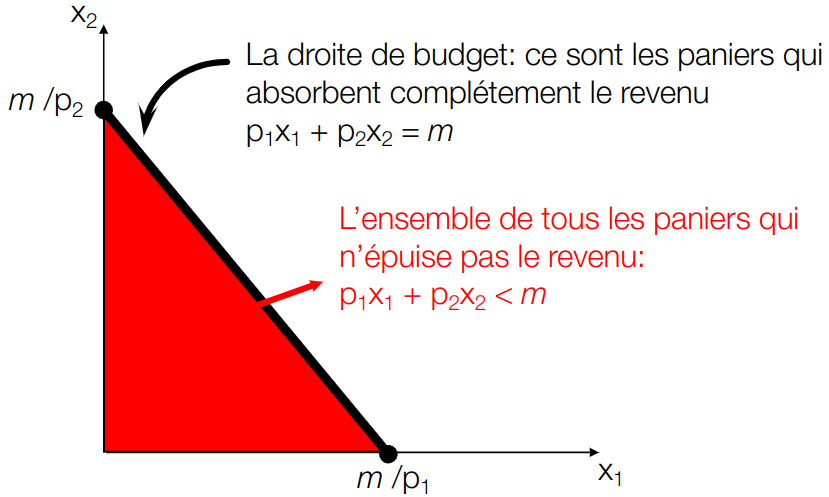
\includegraphics[width=0.4\textwidth,keepaspectratio]{contrainte_budgetaire}
\end{figure}

\subsection{Pente de la droite de budget}

Elle a une représentation économique intéressante : elle mesure le coût d’opportunité de la consommation du bien 1 (taux auquel le consommateur est prêt à substituer le bien 1 au bien 2).
\begin{itemize}
\item[$\rightarrow$] Pour consommer une unité supplémentaire de bien 1, il faut renoncer à $\frac{p_1}{p_2}$ unités de bien 2.
\end{itemize}

\subsection{Déplacement de la droite de budget}

\subsubsection{Variation du revenu}
Déplacement parallèle vers le haut si $m \nearrow$, vers le bas si $m \searrow$

\subsubsection{Variation des prix}
Si $p_1$ diminue, la pente diminue et inversement.

\section{Préférences}

\textbf{Panier de biens} : ensemble composé d'un ou de plusieurs produits, représentés par un vecteur $X = (x_1, x_2)$ indiquant la quantité de chacun de ces biens et services.

\textbf{Préférences} : caractérisent comment chaque individu ordonne les alternatives (panier) possibles.
On peut :
\begin{itemize}
\item Préférer strictement $a$ à $b$ (ou l'inverse) : $a \succ b$ ($a \prec b$)
\item Être indifférent entre $a$ et $b$ : $a \sim b$
\item Préférer faiblement $a$ à $b$ (ou l'inverse) : $a \succeq b$ ($a \preceq b$)
\end{itemize}

\subsection{Hypothèse sur les relations de préférences}

\begin{enumerate}
\item \textblue{Complètes} : le consommateur est toujours capable de faire un choix entre 2 paniers
\item \textblue{Réflexives} : tout panier $X$ est au moins aussi désirable que lui-même
\item \textblue{Transitives} : si $a \succeq b$ et $b \succeq c$, alors $a \succeq c$ 
\item \textblue{Monotones} : si par rapport à un panier $Y$, un panier $X$ a une quantité plus importante d'au moins un bien et pas moins de l'autre bien, les pentes des Courbes d'Indifférences (\textit{CI}) seront négatives, et :
	\begin{itemize}
	\item $X \succeq Y$ si les préférences sont faiblement monotones
	\item $X \succ Y$ si les différences sont strictement monotones
	\end{itemize}
\item \textblue{Convexes} : les consommateurs apprécient la diversité et ils préfèrent les paniers intermédiaires aux paniers extrêmes.
\end{enumerate}
$\Longrightarrow$ les préférences normales respectent ces 5 hypothèses.

\subsection{Courbes d'indifférences}

La CI passant par un panier $X$ est composée de tous les paniers laissant le consommateur indifférent à ce panier $X$.

Un panier situé sur une CI plus élevée qu'un autre est strictement préféré à ce dernier $\rightarrow$ deux CI ne peuvent donc pas se croiser.

Graphiquement, si on prend 2 paniers $X$ et $Y$ ($X \sim Y$), toutes les combinaisons convexes de $X$ et $Y$ sont situées sur le segment de droite $[X, Y]$. La convexité des préférences implique que : 
\begin{itemize}
\item Aucun point de ce segment ne se trouve sous la courbe d'indifférence (la CI ne peut dont être une droite).
\item Si la convexité est stricte : tout le segment de droite se situe au-dessus de la CI passant par $X$ et $Y$. Les CI sont alors nécessairement convexes par rapport à l'origine.
\end{itemize}

\subsection{Exemples de préférences}

\subsubsection{Substituts parfaits}

Disposé à substituer un bien par l’autre à un taux constant. La pente vaut -1.
\begin{figure}[H]
	\centering
	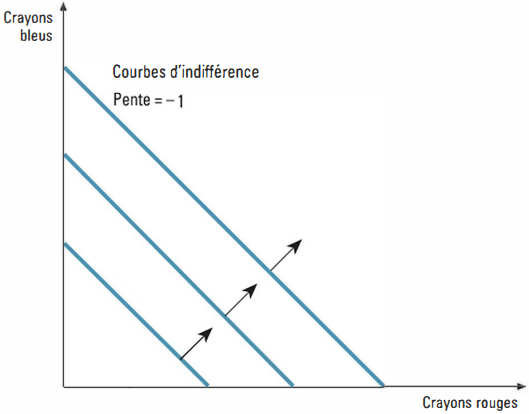
\includegraphics[width=0.4\textwidth,keepaspectratio]{subsituts_parfaits}
\end{figure}

\subsubsection{Compléments parfaits}

Toujours consommés dans des proportions fixes.
\begin{figure}[H]
	\centering
	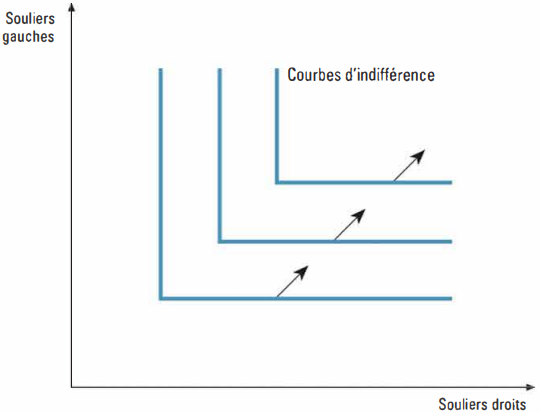
\includegraphics[width=0.4\textwidth,keepaspectratio]{complements_parfaits}
\end{figure}


\subsubsection{Biens indésirables}

Prenons un point $(x_1, x_2)$, un certain nombre de poivrons et d’anchois. Si nous donnons au consommateur quelques anchois supplémentaires, comment devons-nous modifier la quantité de poivrons pour maintenir le consommateur sur la même CI ? Nous devons lui en donner quelques-uns en plus en échange des anchois supplémentaires. La pente est positive.
\begin{figure}[H]
	\centering
	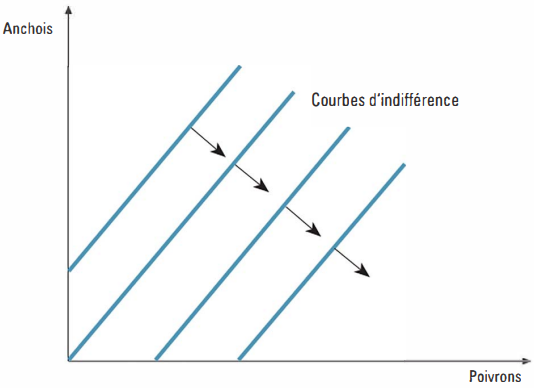
\includegraphics[width=0.4\textwidth,keepaspectratio]{biens_indesirables}
\end{figure}

\subsubsection{Bien neutre}

Le consommateur ne se préoccupe pas du tout du bien 2 (anchois).
\begin{figure}[H]
	\centering
	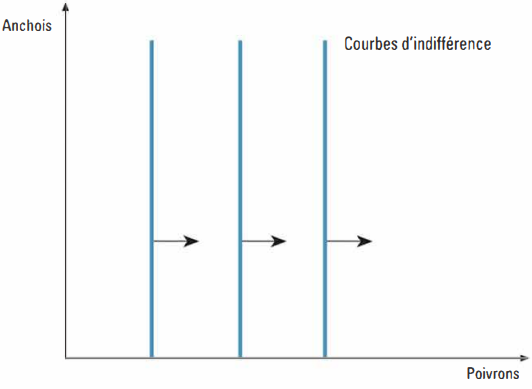
\includegraphics[width=0.4\textwidth,keepaspectratio]{bien_neutre}
\end{figure}

\newpage
\subsubsection{Saturation}

Un point $(x_1,x_2)$ est strictement préféré à tous les autres → plus on s’en éloigne, moins on est satisfait.
\begin{figure}[H]
	\centering
	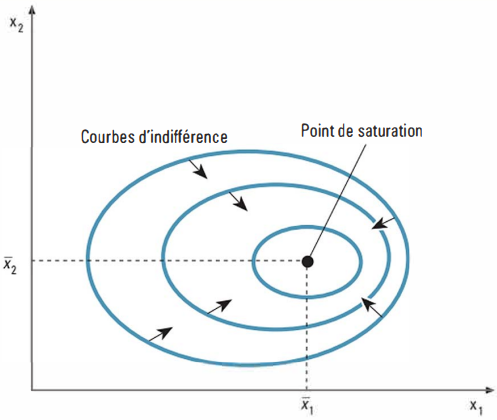
\includegraphics[width=0.4\textwidth,keepaspectratio]{saturation}
\end{figure}

\subsection{Taux Marginal de Substitution (TmS)}

Le TmS mesure la pente de la courbe d'indifférence : $\frac{\Delta x_2}{\Delta x_1}$. Il représente le taux pour lequel le consommateur est indifférent à une substitution de bien 1 au bien 2 (mesure la propension marginale à payer).

\section{L'Utilité}

L'utilité sert à représenter l'ordre dans lequel le consommateur classe les différentes alternatives en fonction de ses préférences.

\begin{enumerate}
\item \textblue{Utilité ordinale} : utilisée ici car on ne se préoccupe que de l'ordre, du classement des préférences. Les valeurs numériques des niveaux d'utilité n'ont pas de signification intrinsèque.
\item \textblue{Utilité cardinale} : la grandeur de l'écart entre les niveaux d'utilité est censée avoir une certaine signification.
\end{enumerate}

\subsection{Fonction d'utilité}

Elle associe à chaque panier une valeur réelle de sorte que si $X \succ Y$, la valeur associée à $X$ ($u(X)$) $>$ à celle associée à $Y$ ($u(Y)$).

Le taux de variation de$f(u)$ peut être mesurée par : $\frac{f(u_1)-f(u_2)}{u_1 - u_2}$. Il sera toujours positif étant donné que le dénominateur auront toujours le même signe.

\subsection{Déterminer les CI à partir d'une fonction d'utilité}

Les paniers situés sur la même Ci ont la même valeur et ceux situés sur des CI supérieures auront des valeurs plus élevées (seul les préférences normales peuvent être représentées par une fonction d'utilité).

\textbf{CI} = ensemble de valeurs $x_1$ et $x_2$ telles que $k = x_1 + x_2$.

\subsection{Exemples de fonctions d'utilité}

\begin{itemize}
\item \textblue{Substituts parfaits} : $u(x_1,x_2) = ax_1 + bx_2$
\item \textblue{Compléments parfaits} : $u(x_1,x_2) = min\{x_1,x_2\}$
\item \textblue{Préférences quasi-linéaires} : $u(x_1,x_2) = f(x_1) + x_2$
\item \textblue{Préférences de Cobb-Douglas} : $u(x_1,x_2) = Ax^c_1x^d_2$ avec $c,d > 0$.
Ici, les CI sont strictement monotones et strictement convexes. Il est toujours possible de trouver une transformation monotone de la fonction qui rende la somme $c+d=1$.
\end{itemize}

\subsection{Utilité marginale}

Variation d'utilité de l'individu lorsqu'il reçoit un peu plus du bien $i$
\begin{equation*}
Um_i = \frac{\Delta u}{\Delta x_i} = \frac{\delta u}{\delta x_i}
\end{equation*}

On peut utiliser la fonction d'utilité pour mesurer le TmS :
\begin{equation*}
TmS = -\frac{Um_1}{Um_2}
\end{equation*}

\section{Le choix}

\textbf{Le choix optimal} : point de tangence entre la CI la plus haute et la droite de budget.
\begin{equation*}
|TmS(x^*_1,x^*_2)| = \frac{p_1}{p_2}
\end{equation*}
\begin{figure}[H]
	\centering
	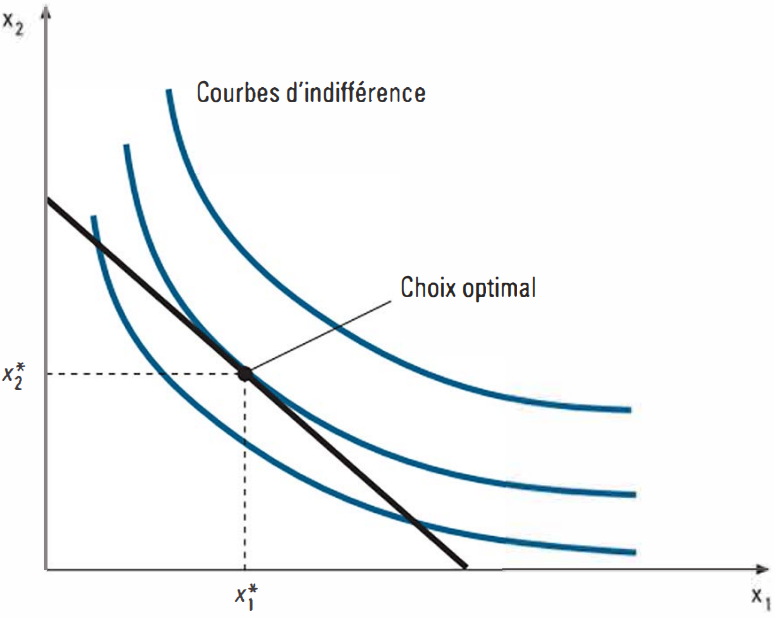
\includegraphics[width=0.4\textwidth,keepaspectratio]{choix_optimal}
\end{figure}

\subsection{2 types de solutions}

\begin{enumerate}
\item Solution intérieure : si $x^*_1 > 0$ et $x^*_2 > 0$, le choix de ($x^*_1,x^*_2$) épuise complètement le budget.
\item Solution de coin : la consommation d'un des biens est nulle.
\end{enumerate}

\subsection{La demande du consommateur}

Panier demandé par le consommateur = quantités optimales de biens 1 et 2. Les fonctions de demande dépendent des prix et du revenu :
\begin{equation*}
x_1(p_1,p_2,m) \text{ } x_2(p_1,p_2,m)
\end{equation*}

\subsection{Fonctions de demande}

\subsubsection{Cobb-Douglas}
\begin{equation*}
x^*_1(p_1,p_2,m) = \frac{am}{(a+b)p_1}
\end{equation*}

\subsubsection{Compléments parfaits}
\begin{equation*}
x^*_1 = x^*_2 = \frac{m}{p_1+p_2}
\end{equation*}

\subsubsection{Substituts parfaits}

\begin{equation*}
x^*_1(p_1,p_2,m) =
\begin{cases}
	0 &\text{ si } p_1 > p_2\\
	[0, \frac{m}{p_1}] &\text{ si } p_1 = p_2\\
	\frac{m}{p_1} &\text{ si } p_1 < p_2
\end{cases}
\text{, }
x^*_2(p_1,p_2,m) =
\begin{cases}
	0 &\text{ si } p_1 < p_2\\
	[0, \frac{m}{p_2}] &\text{ si } p_1 = p_2\\
	\frac{m}{p_2} &\text{ si } p_1 > p_2
\end{cases}
\end{equation*}

\subsubsection{Préférences quasi-linéaires}

Utiliser le Lagrangien ou :
\begin{enumerate}
\item Résoudre une solution intérieure avec $TmS = \frac{p_1}{p_2}$ pour le bien 1 ou 2
\item Trouver la solution pour l'autre bien avec la contrainte de budget
\item Pour avoir une solution intérieure, les deux doivent être > 0 $\rightarrow$ en déduire si c'est une solution de coin ou intérieure (si $\frac{Um_1}{p_1} > \frac{Um_2}{p_2}, x_1 > 0$ et $x_2 = 0$
\item Si c'est une solution de coin :
\begin{itemize}
\item Pour le bien 1 : $(\frac{m}{p_1}, 0)$
\item Pour le bien 2 : $(0, \frac{m}{p_2}$
\end{itemize}
\end{enumerate}

\subsubsection{Conclusion}

\begin{itemize}
\item La contrainte de budget sera toujours effective
\item Le consommateur préfère toujours consommer davantage, il dépense l'intégralité de $m$
\item La demande est homogène de degré 0 : lorsqu'on multiplie tous les prix et le revenue par une constante $t > 0$, la demande ne change pas
\end{itemize}

\section{La demande}

\textbf{Statique comparative} : étudier comment un choix se modifie suite à un changement dans l'environnement économique.

\subsection{Modification du revenu}

\subsubsection{Chemin d'expansion du revenu}

Droite/courbe reliant les paniers demandés à chaque niveau de revenu

\begin{figure}[H]
	\centering
	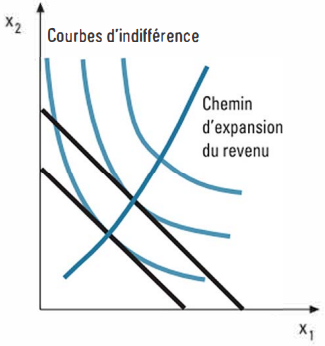
\includegraphics[width=0.27\textwidth,keepaspectratio]{chemin_expansion_revenu}
\end{figure}

\subsubsection{Courbe d'Engel}

Représentation de la demande d'un des biens en fonction du revenu avec les prix constants (revient à isoler $m$)

\begin{figure}[H]
	\centering
	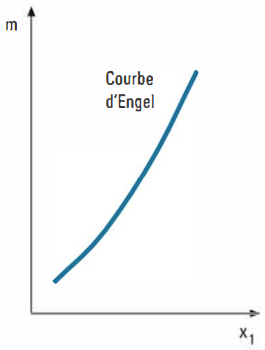
\includegraphics[width=0.24\textwidth,keepaspectratio]{courbe_engel}
\end{figure}

\subsection{Types de biens}

\begin{itemize}
\item  Bien normal : sa demande $\nearrow$ si $m$ $\nearrow$ et inversement. Donc $\frac{\Delta x}{\Delta m} > 0$
\item Bien inférieur : sa demande $\searrow$ si $m$ $\nearrow$. Donc $\frac{\Delta x}{\Delta m} < 0$
\end{itemize}

\begin{minipage}{0.48\textwidth}
	\begin{figure}[H]
		\centering
		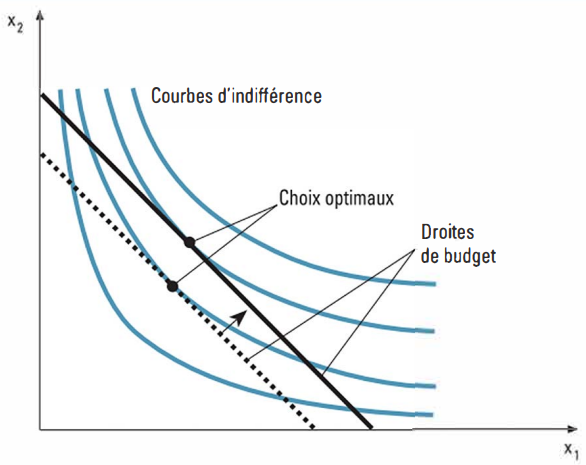
\includegraphics[width=0.8\textwidth,keepaspectratio]{biens_normaux}
		\legend{Biens normaux}
	\end{figure}
\end{minipage}
\begin{minipage}{0.5\textwidth}
	\begin{figure}[H]
		\centering
		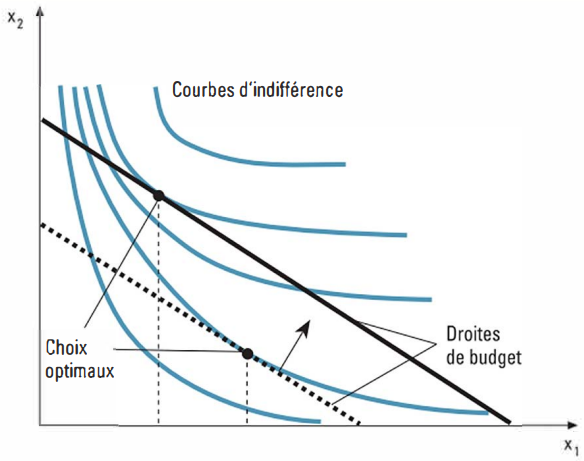
\includegraphics[width=0.8\textwidth,keepaspectratio]{bien_inferieur}
		\legend{Bien inférieur}
	\end{figure}
\end{minipage}

\subsection{Exemples}

\subsubsection{Substituts parfaits}

Ici pour $p_1 < p_2$ (inverse si $p_1 > p_2$)
\begin{figure}[H]
	\centering
	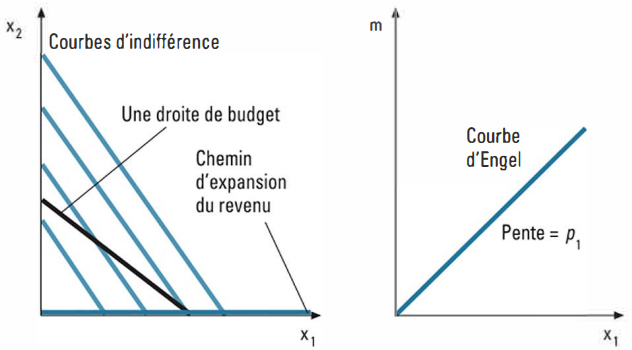
\includegraphics[width=0.5\textwidth,keepaspectratio]{substituts_parfaits_expansion}
\end{figure}

\subsubsection{Compléments parfaits}

\begin{figure}[H]
	\centering
	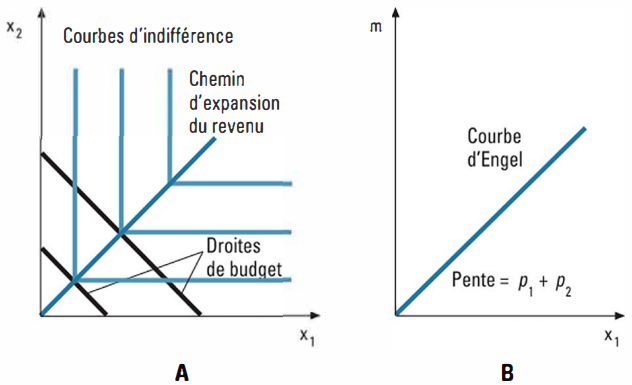
\includegraphics[width=0.5\textwidth,keepaspectratio]{complements_parfaits_expansion}
\end{figure}

\subsubsection{Cobb-Douglas}

\begin{figure}[H]
	\centering
	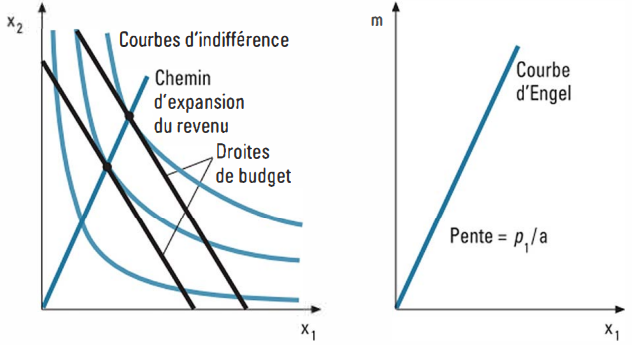
\includegraphics[width=0.5\textwidth,keepaspectratio]{preference_cobb_douglas}
\end{figure}

\subsubsection{Préférences homothétiques}

Biens dont la demande croît dans la même proportion que le revenu. Les substituts parfaits, les compléments parfaits et les préférences de Cobb-Douglas en font partie. Le chemin d'expansion du revenu est alors une ligne droite partant de l'origine.

\paragraph{Bien de luxe}

La demande croît proportionnellement plus que le revenu

\paragraph{Bien de nécessité}

La demande croît proportionnellement moins que le revenu

\subsubsection{Préférences quasi-linéaires}

Elles ne sont pas homothétiques. Le revenu augmente mais la quantité de bien 1 reste la même et tout le revenu supplémentaire est dépensé en bien 2.

\begin{figure}[H]
	\centering
	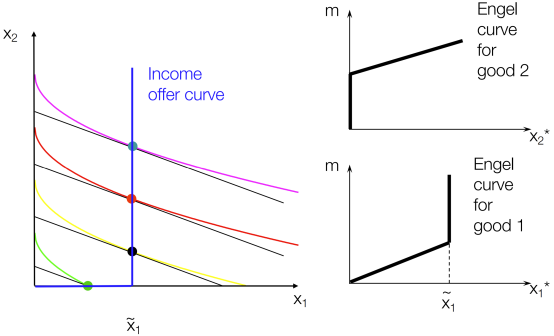
\includegraphics[width=0.5\textwidth,keepaspectratio]{preference_quasi_lineaire_expansion}
\end{figure}

\subsection{Modification des prix}

Si on décide de fixer $p_2$ et $m$, et de modifier $p_1$ :

\subsubsection{Pour un bien ordinaire}

La demande $\nearrow$ quand son prix $\searrow$
\begin{figure}[H]
	\centering
	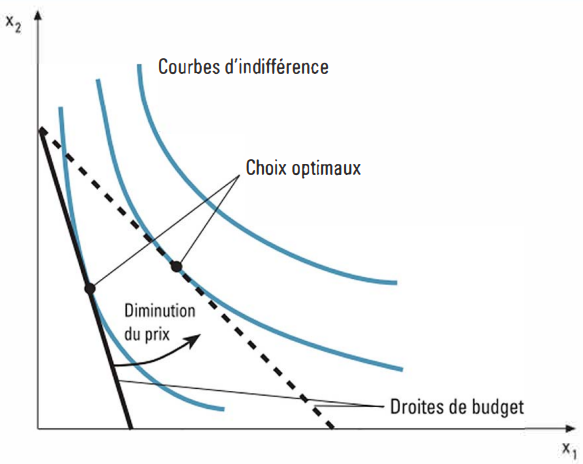
\includegraphics[width=0.5\textwidth,keepaspectratio]{diminution_bien_ordinaire}
\end{figure}


\subsubsection{Pour un bien de Giffen}

La demande $\searrow$ quand son prix $\searrow$
\begin{figure}[H]
	\centering
	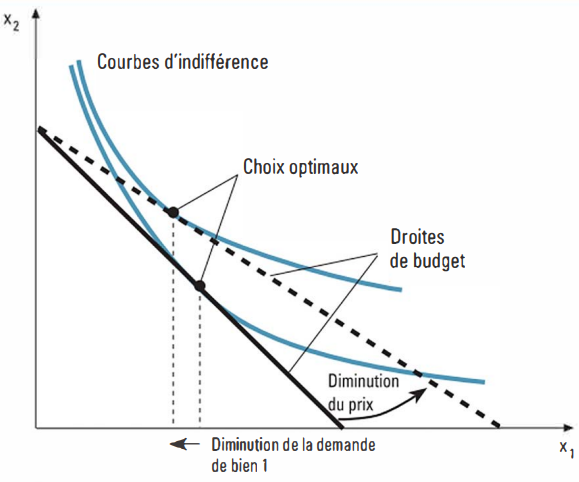
\includegraphics[width=0.5\textwidth,keepaspectratio]{diminution_bien_giffen}
\end{figure}

\subsection{Chemin d'expansion du prix et courbe de demande}

Le prix et la quantité d'un bien varient en sens opposés : la courbe de demande a généralement une pente négative sauf pour un bien de Giffen ou la pente est positive (cas très rare).
\begin{figure}[H]
	\centering
	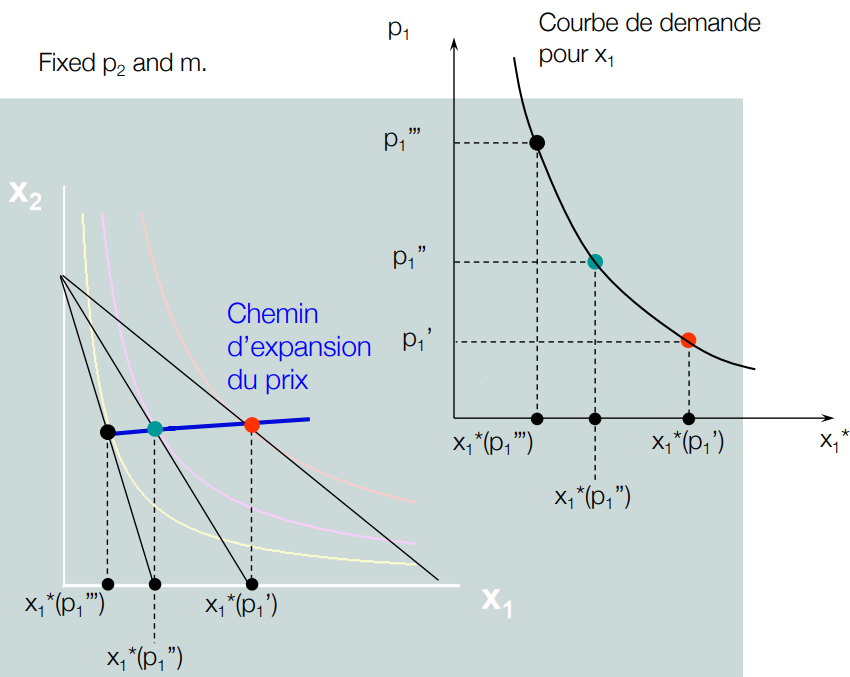
\includegraphics[width=0.5\textwidth,keepaspectratio]{chemin_expansion_courbe_demande}
\end{figure}

\subsubsection{Substituts parfaits}

\begin{figure}[H]
	\centering
	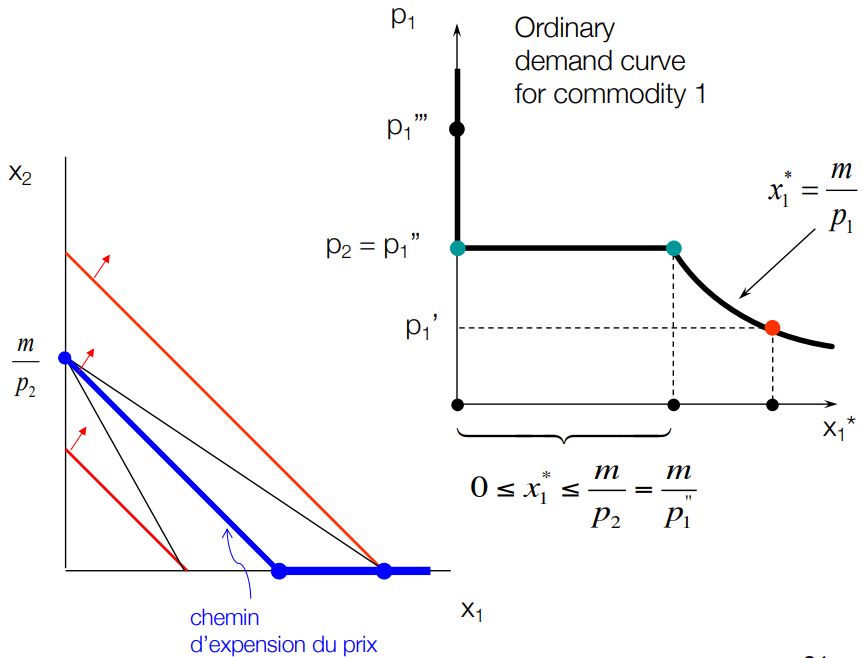
\includegraphics[width=0.4\textwidth,keepaspectratio]{chemin_expansion_courbe_demande_substituts_parfaits}
\end{figure}

\subsubsection{Compléments parfaits}

\begin{figure}[H]
	\centering
	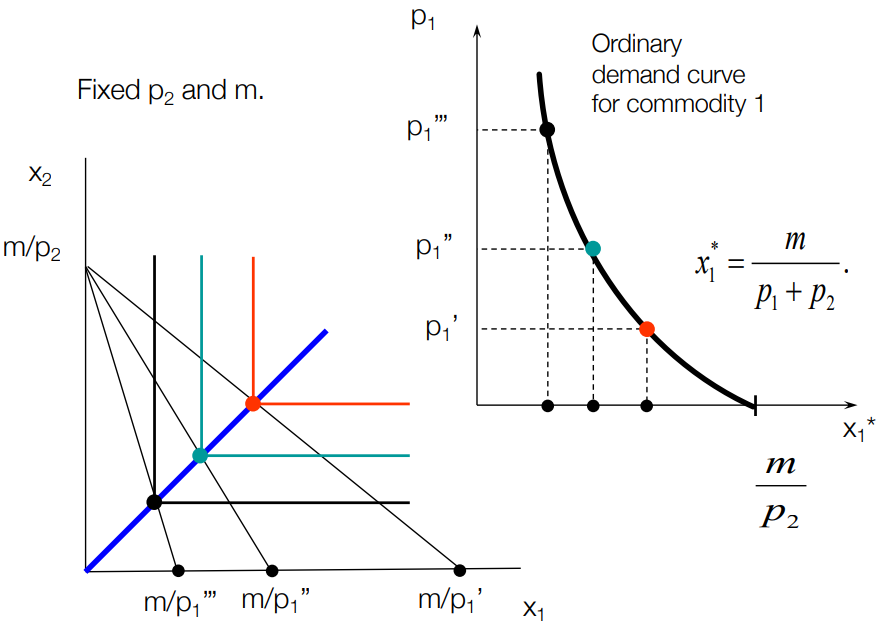
\includegraphics[width=0.4\textwidth,keepaspectratio]{chemin_expansion_courbe_demande_complements_parfaits}
\end{figure}

\subsection{Fonction de demande inverse}

Elle exprime le prix en fonction de la quantité. Pour chaque niveau de demande de bien 1, la fonction de demande inverse mesure le prix du bien 1 nécessaire pour que le consommateur choisisse ce niveau de consommation. La hauteur de la courbe de demande pour un niveau donné de consommation mesure la propension marginale à payer pour une unité additionnelle du bien à ce niveau de consommation.

\section{Évolution de la demande en fonction du prix : effet de revenu et de substitution}

But : étudier la variation d'un bien sur le choix du consommateur.

\subsection{2 effets}

\begin{itemize}
\item \textblue{Effet de substitution} : variation de la demande due à une \textred{modification du taux d'échange entre les deux bien}.
\item \textblue{Effet de revenu} : variation de la demande due à une \textred{modification du pouvoir d'achat}.
\end{itemize}

\newpage
\subsection{Méthode de Slutsky}

\begin{enumerate}
\item Considérer uniquement la variation des prix relatifs en ajustant le revenu nominal pour maintenir le pouvoir d'achat constant
	\begin{itemize}
	\item[$\rightarrow$] Rotation de la droite de budget autour du panier initial $X$, la pente de la droite de budget change et on passe au panier $Y$
	\item[$\Rightarrow$] Quand le prix d'un bien décroît, nous devons diminuer le revenu de façon à maintenir le pouvoir d'achat constant.
	\end{itemize}
\item Laisser le pouvoir d'achat se modifier en maintenant les prix relatifs constants
	\begin{itemize}
	\item[$\rightarrow$] Déplacement parallèle vers le haut, la pente reste constante et c'est le pouvoir d'achat qui se modifie. On passe de $m'$ à $m$, et du panier $Y$ au panier $Z$.
	\end{itemize}
\end{enumerate}

\begin{figure}[H]
	\centering
	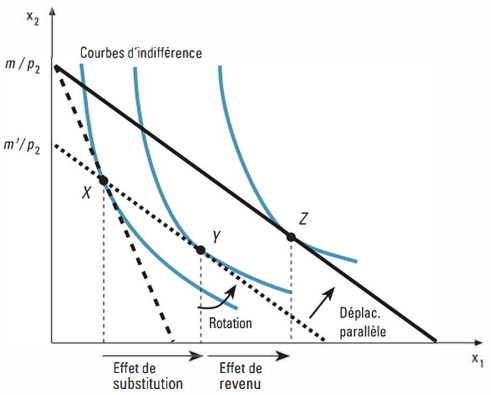
\includegraphics[width=0.4\textwidth,keepaspectratio]{slutsky}
\end{figure}


\subsection{Différents types de biens}

\subsubsection{Biens normaux}
Une diminution du revenu entraîne une diminution de la demande.
\begin{figure}[H]
	\centering
	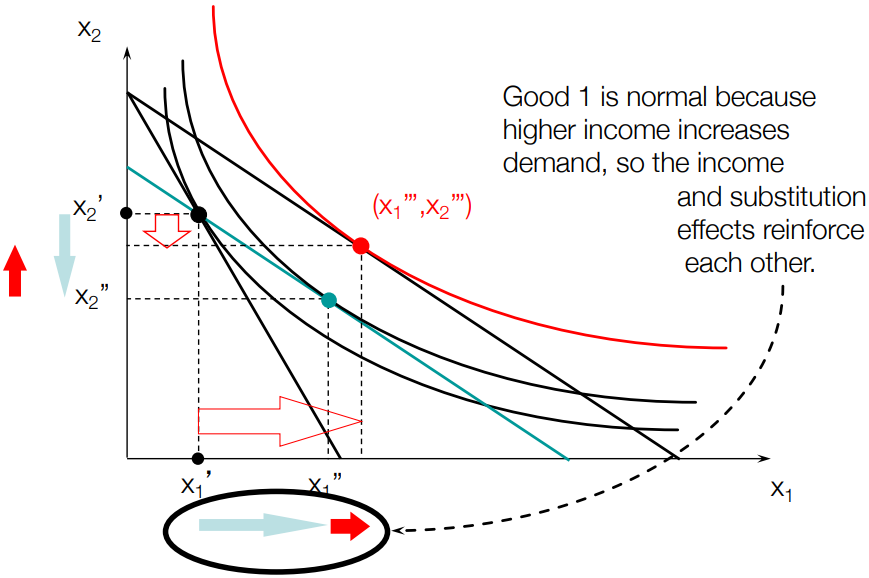
\includegraphics[width=0.4\textwidth,keepaspectratio]{slutsky_bien_normal}
\end{figure}

\subsubsection{Biens inférieurs}
Une diminution du revenu entraîne une augmentation de la demande. les effets de substitution et de revenu s'opposent car l'effet de revenu est dans la direction opposées.
\begin{figure}[H]
	\centering
	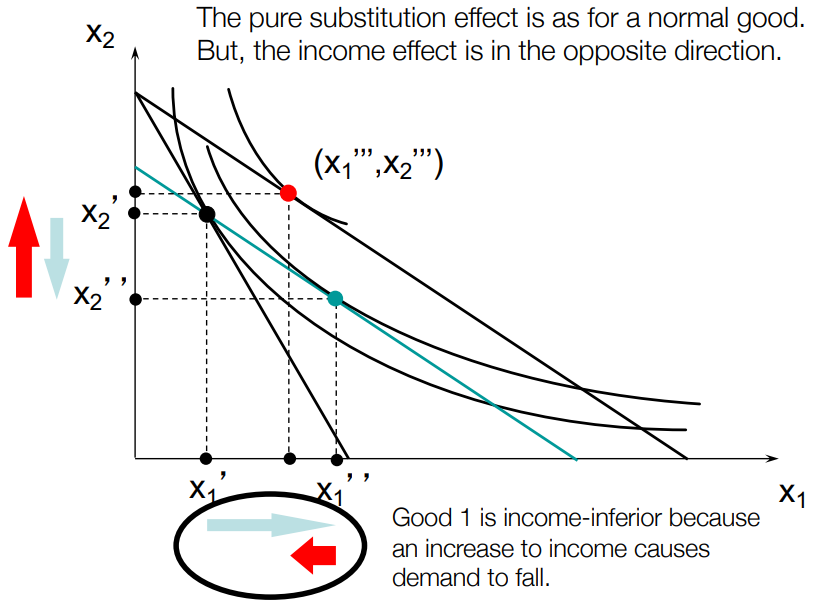
\includegraphics[width=0.4\textwidth,keepaspectratio]{slutsky_bien_inferieur}
\end{figure}

\subsubsection{Biens de Giffen}
L'effet dde revenu est supérieur à l'effet de substitution, la quantité finale demandée diminue.
\begin{figure}[H]
	\centering
	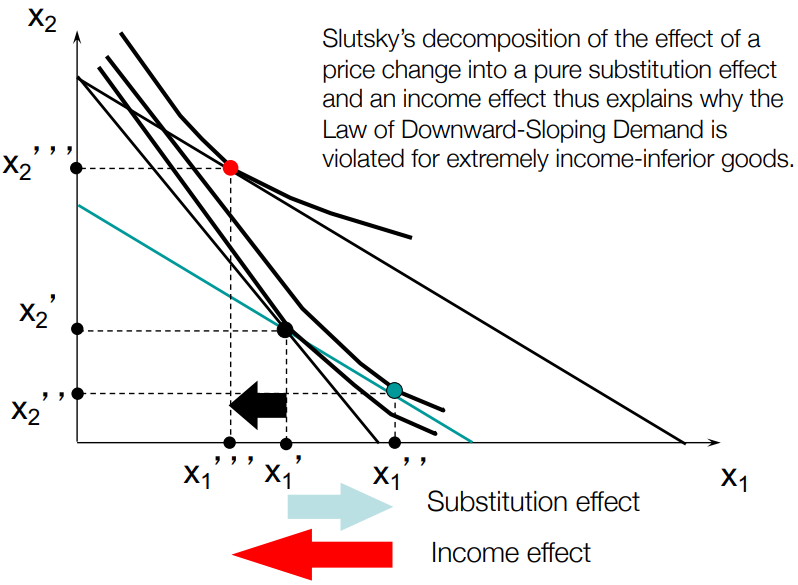
\includegraphics[width=0.4\textwidth,keepaspectratio]{slutsky_bien_giffen}
\end{figure}

\subsection{Effet de substitution de Hicks}
Supposons qu'au lieu de faire pivoter la droite de budget autour du panier initial de consommation, nus la faisions rouler le long de la CI passant par le panier initial. nous considérons ainsi un consommateur confronté à une nouvelle droite de budget finale mais à un revenu différent. le pouvoir d'achat associé à cette nouvelle droite ne permet plus d'acheter le panier initial, mais il permet d'acquérir un panier qui lui est indifférent.

\begin{figure}[H]
	\centering
	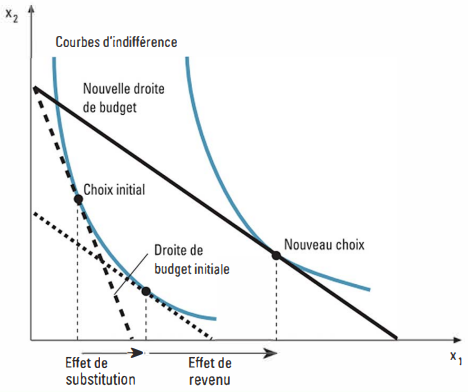
\includegraphics[width=0.4\textwidth,keepaspectratio]{substitution_hicks}
\end{figure}

\begin{enumerate}
\item Maintient l'utilité constante au lieu du pouvoir d'achat
\item \textblue{L'effet de substitution de Slutsky} donne au consommateur une somme d'argent qui lui permet de \textred{retourner à son niveau initial de consommation} alors que l'effet de substitution de Hicks lui donne une somme qui lui permet de \textred{rester sur sa CI initiale}.
\end{enumerate}

\section{L'incertitude}

il existe plusieurs états du monde possible mais l'état qui se réalisera est inconnu lors de la prise de décision $\rightarrow$ conséquences incertaines. On associe un résultat à chaque état du monde.

Ici, on suppose que l'agent économique connaît tous les états du monde possibles et la probabilité de réalisation de chacun de ces états du monde (incertitude probabilisable). Évidemment, un seul des résultats possibles va se réaliser.

\subsection{Loteries}

\begin{itemize}
\item Manière de modéliser les actions : choix de loteries
\item loterie : distribution de probabilités sur un ensemble de résultats possibles
\item Loterie certaine : $\mathcal{L} = (1|x_1)$
\end{itemize}

\begin{equation*}
\displaystyle\sum_{i=1}^{n} \pi_i = 1
\end{equation*}
